\documentclass[aspectratio=169, 10pt]{beamer}

\usepackage{bm} % bold math
\usepackage{fontspec}
\usepackage{minted}
\usepackage{pgf-pie}
\usepackage{tikz}

% Custom commands and environments
\makeatletter
\newcommand\version[1]{\renewcommand\@version{#1}}
\newcommand\@version{}
\def\insertversion{\@version}

\newcommand\course[1]{\renewcommand\@course{#1}}
\newcommand\@course{}
\def\insertcourse{\@course}

\newcommand\coursetitle[1]{\renewcommand\@coursetitle{#1}}
\newcommand\@coursetitle{}
\def\insertcoursetitle{\@coursetitle}

\newcommand\lecturenumber[1]{\renewcommand\@lecturenumber{#1}}
\newcommand\@lecturenumber{}
\def\insertlecturenumber{\@lecturenumber}
\makeatother

\newcommand{\slidetitle}[1]{{\xbseries \large \structure{#1}} \bigskip}
\newcommand{\term}[1]{{\color{blue} #1}}
\newcommand{\leftspace}{\hspace{1em}}
\newcommand{\inlinearrow}{
  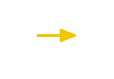
\begin{tikzpicture}[baseline]
    \node [anchor=base] (x) {};
    \draw [rawarrow] (x.mid west) -- ($(x.mid west) + (2em,0)$);
  \end{tikzpicture}
}

\newenvironment{slide}
{\begin{frame}[fragile,environment=slide]\vskip0pt plus 1filll}
{\vskip0pt plus 1filll\end{frame}}

% LaTeX

\setlength{\leftmargini}{1em}

% Common Information

\author{Jon Eyolfson}
\course{ECE 353}
\coursetitle{Systems Software}
\date{2024 Winter}

% fontspec

\defaultfontfeatures{Ligatures=TeX}
% \setmainfont{Domine}
\setsansfont{Inter}[
  FontFace={ul}{n}{Font=*-Thin},
  FontFace={el}{n}{Font=*-ExtraLight},
  FontFace={l}{n}{Font=*-Light},
  FontFace={sb}{n}{Font=*-SemiBold},
  FontFace={eb}{n}{Font=*-ExtraBold},
  FontFace={xb}{n}{Font=*-Black},
]
\setmonofont[Contextuals=AlternateOff, Ligatures=TeXOff]{Iosevka}[
  FontFace={xb}{n}{Font=*-Heavy},
]

%% Font Weights

\DeclareRobustCommand{\ulseries}{\fontseries{ul}\selectfont}
\DeclareTextFontCommand{\textul}{\ulseries}
\DeclareRobustCommand{\elseries}{\fontseries{el}\selectfont}
\DeclareTextFontCommand{\textel}{\elseries}
\DeclareRobustCommand{\lseries}{\fontseries{l}\selectfont}
\DeclareTextFontCommand{\textl}{\lseries}
\DeclareRobustCommand{\sbseries}{\fontseries{sb}\selectfont}
\DeclareTextFontCommand{\textsb}{\sbseries}
\DeclareRobustCommand{\ebseries}{\fontseries{eb}\selectfont}
\DeclareTextFontCommand{\texteb}{\ebseries}
\DeclareRobustCommand{\xbseries}{\fontseries{xb}\selectfont}
\DeclareTextFontCommand{\textxb}{\xbseries}

% tikz

\usetikzlibrary{
  arrows,
  arrows.meta,
  automata,
  backgrounds,
  calc,
  decorations.pathreplacing,
  matrix,
  positioning,
  overlay-beamer-styles,
  shapes,
  shapes.multipart,
  tikzmark,
}

\tikzstyle{rawarrow} = [
  -{Latex[round]},
  line width=1pt,
  yellow,
  shorten >=3pt,
  shorten <=3pt,
  font=\small,
  text=black,
]

\tikzstyle{arrow} = [
  -{Latex[round]},
  line width=1pt,
  yellow,
  shorten >=3pt,
  shorten <=3pt,
  transform canvas={yshift=3pt},
  font=\small,
  text=black,
]

\newcommand{\tikzmarkcoord}[1]{([yshift=3pt]pic cs:#1)}

% minted

\setminted{style=eyolfson, fontsize=\small, escapeinside=||}
\setmintedinline{fontsize=\normalsize}

% hyperref

\hypersetup{colorlinks, urlcolor=blue}

% beamer
\setbeamersize{text margin left=16mm, text margin right=16mm}
\setbeamertemplate{itemize items}[circle]
\setbeamercolor{item}{fg=black}
\setbeamercolor{structure}{fg=darkblue}
\setbeamerfont{frametitle}{series=\bfseries, parent=structure}
\setbeamertemplate{navigation symbols}{}
\setbeamertemplate{headline}{}
\setbeamertemplate{footline}{
  \begin{tikzpicture}[
    remember picture,
    overlay,
    shift={(current page.south west)},
  ]
    \path [fill=gray] (144mm, 0) -- (160mm, 16mm) -- (160mm, 0);
    \node [inner sep=3.5mm, outer sep=0, text=black, anchor=base east,
           align=right, yshift=3.5mm]
          at (current page.south east) {\ttfamily \small \insertframenumber{}};
  \end{tikzpicture}
}
\setbeamertemplate{title page}{
  \begin{tikzpicture}[
    remember picture,
    overlay,
    shift={(current page.south west)},
    background rectangle/.style={fill=darkblue},
    show background rectangle,
  ]
    \node [anchor=center, align=center, text=white, text width=40mm, scale=3.2]
          at (\paperwidth / 2, \paperheight * 2 / 3)
          {\xbseries \inserttitle{}};
    \node [anchor=base west, align=left, inner sep=0, text=white, yshift=2.5mm]
          at (16mm, \paperheight / 3)
          {\insertdate{} \insertcourse{}: \insertcoursetitle{}};
    \node [anchor=base west, align=left, inner sep=0, text=white, yshift=-2.5mm]
          at (16mm, \paperheight / 3)
          {\insertauthor};
    \node [anchor=base east, align=right, inner sep=0, text=white, yshift=2.5mm]
          at (144mm, \paperheight / 3)
          {Lecture \insertlecturenumber{}};
    \node [anchor=base east, align=right, inner sep=0, text=white,
           yshift=-2.5mm]
          at (144mm, \paperheight / 3)
          {\ttfamily \insertversion{}};
    \node [align=center, anchor=south, inner sep=0, text=white, yshift=3.5mm]
          (license) at (\paperwidth / 2, 0)
          {\fontsize{7pt}{7pt}\selectfont This  work is licensed under a
           \href{http://creativecommons.org/licenses/by-sa/4.0/}
                {\color{lightblue} Creative Commons Attribution-ShareAlike 4.0
                 International License}};
  \end{tikzpicture}
}

% xcolor

%% Primary Colour

\definecolor{pantone655}{RGB}{0, 42, 92} % #002a5c
\colorlet{darkblue}{pantone655}

%% Secondary Colours

\definecolor{pantone633}{RGB}{0, 139, 176} % #008bb0
\colorlet{blue}{pantone633}

\definecolor{pantonewarmred}{RGB}{220, 70, 51} % #dc4633
\colorlet{red}{pantonewarmred}

\definecolor{pantone3285}{RGB}{0, 161, 137} % #00a189
\colorlet{cyan}{pantone3285}

\definecolor{pantone7722}{RGB}{13, 83, 77} % #0d534d
\colorlet{darkcyan}{pantone7722}

\definecolor{pantone376}{RGB}{141, 191, 46} % #8dbf2e
\colorlet{green}{pantone376}

\definecolor{pantone2613}{RGB}{109, 36, 122} % #6d247a
\colorlet{violet}{pantone2613}

\definecolor{pantone2985}{RGB}{111, 199, 234} % #6fc7ea
\colorlet{lightblue}{pantone2985}

\definecolor{pantone227}{RGB}{171, 19, 104} % #ab1368
\colorlet{magenta}{pantone227}

\definecolor{pantone7406}{RGB}{241, 197, 0} % #f1c500
\colorlet{yellow}{pantone7406}

%% Neutrals

\definecolor{pantonecoolgray2}{RGB}{208, 209, 201} % #d0d1c9
\colorlet{gray}{pantonecoolgray2}


\lecturenumber{22}
\title{Locks Implementation}
\version{2.0.0}

\begin{document}
  \begin{frame}[plain, noframenumbering]
    \titlepage
  \end{frame}

  \begin{slide}

    \slidetitle{
      You Can Implement Locks in Software
      
      with Minimal Hardware
    }

    Your hardware requirements just have to ensure:
    \begin{itemize}
      \item Loads and stores are atomic
      \item Instructions execute in order
    \end{itemize}
    \medskip

    There are 2 main algorithms you could use:
    
    \leftspace{}\href{https://en.wikipedia.org/wiki/Peterson\%27s_algorithm}
    {Peterson's algorithm}
    and
    \href{http://en.wikipedia.org/wiki/Lamport\%27s_bakery_algorithm}
         {Lamport's bakery algorithm}
    \medskip

    However, they don't scale well, and processors execute
    out-of-order

  \end{slide}

  \begin{slide}

    \slidetitle{Let's Assume a Magical Atomic Function ---
                \texttt{compare\_and\_swap}}

    \texttt{compare\_and\_swap(int *p, int old, int new)} is atomic

    \leftspace{}It returns the original value pointed to

    \leftspace{}It only swaps if the original value equals \texttt{old}, and changes it to \texttt{new}
    \medskip

    Let's give it another shot:

    \begin{minted}[xleftmargin=1em]{c}
void init(int *l) {
  *l = 0;
}
void lock(int *l) {
  while (compare_and_swap(l, 0, 1));
}
void unlock(int *l) {
  *l = 0;
}   
    \end{minted}

  \end{slide}

  \begin{slide}

    \slidetitle{What We Implement is Essentially a Spinlock}

    Compare and swap is a common atomic hardware instruction
    \medskip

    On x86 this is the \texttt{cmpxchg} instruction (compare and exchange)
    \medskip

    However, it still has this ``busy wait'' problem
    \medskip

    Consider a uniprocessor system, if you can't get the lock, you should yield

    \leftspace{}Let the kernel schedule another process, that may free the lock
    \medskip

    On a multiprocessor machine, you could try again

  \end{slide}

  \begin{slide}

    \slidetitle{Let's Add a Yield}

    \begin{minted}{c}
void lock(int *l) {
  while (compare_and_swap(l, 0, 1)) {
    thread_yield();
  }
}
    \end{minted}

    Now we have a 
    \href{https://en.wikipedia.org/wiki/Thundering_herd_problem}{thundering herd}
    problem

    \leftspace{}Multiple threads may be waiting on the same lock
    \medskip

    We have no control over who gets the lock next

    \leftspace{}We need to be able to reason about it (FIFO is okay)

  \end{slide}

  \begin{slide}

    \slidetitle{We Can Add a Wait Queue to the Lock}

    \begin{minted}{c}
void lock(int *l) {
  while (compare_and_swap(l, 0, 1)) {
    // add myself to the lock wait queue
    thread_sleep();
  }
}
void unlock(int *l) {
  *l = 0;
  if (/* threads in wait queue */) {
    // wake up one thread
  }
}
    \end{minted}
    \medskip

    There are 2 issues with this:
    
    \begin{enumerate}
      \item lost wakeup, and
      \item the wrong thread gets the lock
    \end{enumerate}
  \end{slide}

  \begin{slide}

    \slidetitle{Lost Wakeup Example}

    \begin{minted}[linenos]{c}
void lock(int *l) {
  while (compare_and_swap(l, 0, 1)) {
    // add myself to the wait queue
    thread_sleep();
  }
}
void unlock(int *l) {
  *l = 0;
  if (/* threads in wait queue */) {
    // wake up one thread
  }
}
    \end{minted}
    \medskip

    Assume we have thread 1 (T1) and thread 2 (T2), thread 2 holds the lock

    \leftspace{}T1 runs line 2 and fails, swap to T2 that runs lines 10-12, T1
    runs lines 3 -4

    \leftspace{}\leftspace{}T1 will never get woken up!
  \end{slide}

  \begin{slide}

    \slidetitle{Wrong Thread Getting the Lock Example}

    \begin{minted}[linenos]{c}
void lock(int *l) {
  while (compare_and_swap(l, 0, 1)) {
    // add myself to the wait queue
    thread_sleep();
  }
}
void unlock(int *l) {
  *l = 0;
  if (/* threads in wait queue */) {
    // wake up one thread
  }
}
    \end{minted}
    \medskip

    Assume we have T1, T2, and T3. T2 holds the lock, T3 is in queue.

    \leftspace{}T2 runs line 9, swap to T1 which runs line 2 and succeeds

    \leftspace{}\leftspace{}T1 just stole the lock from T3!
  \end{slide}

  \begin{slide}

    \slidetitle{We Can Use Two Variables to Fix This (One to Guard)}

    \begin{columns}
      \begin{column}{0.5\textwidth}
        \begin{minted}{c}
typedef struct { int lock; int guard;
                 queue_t *q; } mutex_t;

void lock(mutex_t *m) {
  while (
    compare_and_swap(m->guard, 0, 1)
  );
  if (m->lock == 0) {
    m->lock = 1; // acquire mutex
    m->guard = 0;
  } else {
    enqueue(m->q, self);
    m->guard = 0;
    thread_sleep();
    // wakeup transfers the lock here
  }
}
        \end{minted}
      \end{column}
      \begin{column}{0.5\textwidth}
        \begin{minted}{c}
void unlock(mutex_t *m) {
  while (
    compare_and_swap(m->guard, 0, 1)
  );
  if (queue_empty(m->q)) {
    // release lock, no one needs it
    m->lock = 0; 
  }
  else {
    // direct transfer mutex
    // to next thread
    thread_wakeup(dequeue(m->q));
  }
  m->guard = 0;
}
        \end{minted}
      \end{column}
    \end{columns}

  \end{slide}

  \begin{slide}

    \slidetitle{There's STILL A Data Race}

    After a thread calls \texttt{lock}, it could get interrupted right before
    the \texttt{thread\_sleep}
    \medskip

    However, it's been added to the wait queue, so \texttt{thread\_wakeup}

    would try to wake up a thread that's not sleeping yet (we know it's about
    to)
    \medskip

    We could simply retry the call to \texttt{thread\_wakeup}

    until the thread finally calls \texttt{thread\_sleep}

  \end{slide}

  \begin{slide}

    \slidetitle{Remember What Causes a Data Race}

    A data race is when two concurrent actions access the same variable

    and at least one of them is a \textbf{write}
    \medskip

    We could have any many readers as we want

    \leftspace{}We don't need a mutex as long as nothing writes at the same
    time
    \medskip

    We need different lock modes for reading and writing

  \end{slide}

  \begin{slide}

    \slidetitle{Read-Write Locks}

    With mutexes/spinlocks, you have to lock the data,

    \leftspace{}even for a read since you don't know if a write could happen
    \medskip

    Reads can happen in parallel, as long as there's no write
    \medskip

    Multiple threads can hold a read lock ({\tt pthread\_rwlock\_rdlock}),

    \leftspace{}but only one thread may hold a write lock ({\tt pthread\_rwlock\_wrlock})

    \leftspace{}and will wait until the current readers are done

  \end{slide}

  \begin{slide}

    \slidetitle{We Can Use A Guard To Keep Track of Readers}

    \begin{columns}
      \begin{column}{0.5\textwidth}
        \begin{minted}{c}
typedef struct {
  int nreader;
  lock_t guard;
  lock_t lock;
} rwlock_t;

void write_lock(rwlock_t *l) (
  lock(&l->lock);
}

void write_unlock(rwlock_t *l) (
  unlock(&l->lock);
}
        \end{minted}
      \end{column}
      \begin{column}{0.5\textwidth}
        \begin{minted}{c}
void read_lock(rwlock_t *l) (
  lock(&l->guard);
  ++nreader;
  if (nreader == 1) { // first reader
    lock(&l->lock);
  }
  unlock(&l->guard);
}
void read_unlock(rwlock_t *l) (
  lock(&l->guard);
  --nreader;
  if (nreader == 0) { // last reader
    unlock(&l->lock);
  }
  unlock(&l->guard);
}
        \end{minted}
      \end{column}
    \end{columns}

  \end{slide}

  \begin{slide}
    \slidetitle{We Want Critical Sections to Protect Against Data Races}

    We should know what data races are, and how to prevent them:
    \begin{itemize}
      \item Mutex or spinlocks are the most straightforward locks
      \item We need hardware support to implement locks
      \item We need some kernel support for wake up notifications
      \item If we know we have a lot of readers, we should use a read-write lock
    \end{itemize}
  \end{slide}

\end{document}
